% @Author: AnthonyKenny98
% @Date:   2020-02-26 08:22:07
% @Last Modified by:   AnthonyKenny98
% @Last Modified time: 2020-04-06 17:53:24

The second objective of this thesis was to design and implement a functional hardware unit that accelerates the execution of \gls{RRT}. With the bottleneck function having been identified in Chapter 2 as edge collision detection, Chapter 3 details the specification, design, implementation, and analysis of a hardware unit the implements the edge collision function.

\section{Defining the Collision Detection Unit}
\todo[inline]{Needs new title.}

    \subsection{Edge Collision Function}
    \label{subsection:EdgeCollisionFunction}
        To briefly examine the edge collision detection function in general terms; Given an edge $e$, \gls{RRT} finds where $e$ intersects with grids in the \glslong{OGM}. If any of the grids it intersects with are ``occupied'', a collision is returned. 

        % @Author: AnthonyKenny98
% @Date:   2020-04-06 17:52:43
% @Last Modified by:   AnthonyKenny98
% @Last Modified time: 2020-04-06 17:52:43

   
    \subsection{Technical Specifications}
    \label{subsection:HoneyBeeTechSpechs}
        Put simply, the functional unit that implements the edge collision detection function in hardware should have the same rough technical specifications as when the function is defined in software (Section \ref{subsection:EdgeCollisionFunction}). That is, it should take an edge $e$ and an \gls{OGM} and return a boolean value: True, if the edge collides with an obstacle, otherwise False.
        Table \ref{table:HoneyBeeTechSpecs} outlines the required technical specifications for the functional unit.
        % @Author: AnthonyKenny98
% @Date:   2020-03-01 14:11:33
% @Last Modified by:   AnthonyKenny98
% @Last Modified time: 2020-03-01 14:33:00
\begin{table}[H]
\begin{center}
\begin{tabular}{|p{.3\linewidth}|p{.64\linewidth}|}
    \hline
    \textbf{Element}             & \textbf{Description/Justification} \\
    \hline
    \multicolumn{2}{|c|}{Contstraints} \\
    \hline
    Dimension $N$  & $N$ defines the dimension of the cubic configuration space for which the functional unit should take an identically sized \ac{OGM}\\
    \hline
    \multicolumn{2}{|c|}{Inputs} \\
    \hline
    Edge $e$  & An Edge $e$ defined for a \ac{3D} configuration space by two points $\{p1, p2\}$, each defined by a set of \ac{3D} coordinates $\{x,y,z\}$.\\
    \hline
    Space $S$ & In an abstract sense, the edge collision detection function takes Space $S$ as an input. In a more practical sense, the functional unit will take an $N\times N\times N$ Occupancy Grid Map \\
    \hline
    Control Inputs & The functional unit must also have ports for control signals such as clock, reset, start, etc. These are required for adding the unit to a processor. \\
    \multicolumn{2}{|c|}{Outputs} \\ 
    \hline
    Return Value & 1 bit return value: 1 if collision, 0 otherwise.\\
    \hline
    Control Outputs & Output ports for control signals such as idle, done, ready, etc. These are required for adding the unit to a processor. \\
    \hline
\end{tabular}
\caption{Technical Specifications for Edge Collision Detection Unit}
\label{table:HoneyBeeTechSpecs}
\end{center}
\end{table}
\todo[inline, caption={Improve Technical Specifications}]{More detail on control units.}

    \subsection{Performance Specifications}
    \label{subsection:HoneyBeePerfSpechs}
        \todo[inline]{Performance Specifications Functional Unit}

\newpage

\section{HoneyBee}

    % @Author: AnthonyKenny98
% @Date:   2020-04-06 17:19:39
% @Last Modified by:   AnthonyKenny98
% @Last Modified time: 2020-04-06 17:29:38
\begin{figure}[H]
\begin{centering}
\includegraphics[width=0.8\linewidth]{chapters/chapter3/img/MegalongHoneyBee.png}
\mycaption{Megalong Park Honey Bee Pollinating a Weeping Cherry Blossom}{. Photographed by Emma Kenny in the Southern Highlands of New South Wales, Australia}
\end{centering}
\end{figure}

    The honey bee, \textit{Apis mellifera}, has long been renowned for its tireless work ethic. However, the honey bee is rarely given credit for its remarkable navigation and collision avoidance strategies during flight. Recent research\cite{Menzel2005} suggests that honey bees, interestingly enough, explore their workspace randomly in order to find paths from their hive to sources of pollen. Sound familiar? As such, it is quite appropriate that this functional unit, designed to work tirelessly, rapidly and efficiently to execute collision detection computations for robot motion planning, was named \textbf{HoneyBee}. \\

    \todo[inline,caption={More Iterations of HoneyBee Design}]{Note: Currently this report only shows the design/build/measurement of the first pass at designing the functional unit (Designated HoneyBee-A, or HB-A). Final report will detail further iterations.}

    \subsection{Design}
        \subsubsection*{HoneyBee-A Design}
        The first design iteration, designated \gls{HB-A}, was designed to take advantage of the performance improvements associated with pipelining. Figure \ref{fig:pipeline} demonstrates how pipelineing in hardware improves latency. By default, instructions are executed in order, one at a time. Pipelining takes advantage of operations that are independent of each other to reduce the number of clock cycles required to complete a set of instructions. 
        % @Author: AnthonyKenny98
% @Date:   2020-03-01 14:49:32
% @Last Modified by:   AnthonyKenny98
% @Last Modified time: 2020-03-01 14:55:51
\begin{figure}[H]
\begin{center}
    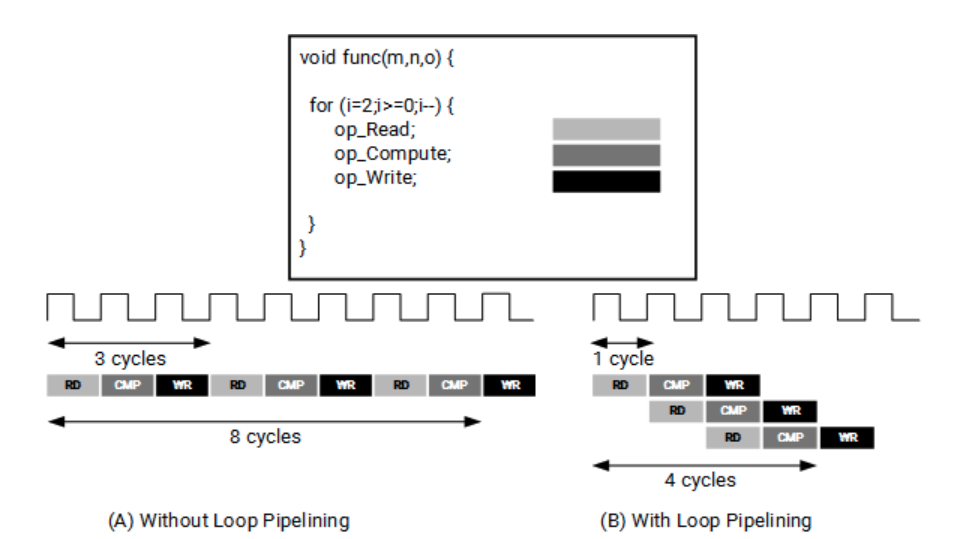
\includegraphics[width=0.9\linewidth]{chapters/chapter3/img/pipeline.png}
    \caption{Pipelining to Improve Latency}
    \label{fig:pipeline}
\end{center}
\end{figure}
\todo[inline]{Make my own version of this figure}
 

    \subsection{Build}
        \subsubsection*{Hardware Description Languages}
        \todo[inline]{Introduction to Hardware Description Languages}

        \subsubsection*{High Level Synthesis}
        \gls{HLS} is an automated hardware design process that takes design files (written in high-level languages, such as C, C++ or SystemC) specifying the algorithmic function of a piece of hardware, interprets those files and creates digital hardware designs that execute this function. It effectively translates programming languages into hardware description languages. Key advantages of using HLS is speed and verification. It is much faster and easier to define functionality in C than it is in a \gls{HDL} such as Verilog, and thus design iterations are faster. It is also much simpler to verify one's design, as the functional units can be put through test benches written in C. This project used Vivado HLS to build the HoneyBee Unit.

        \subsubsection*{HoneyBee-A Synthesis}
        Figure \ref{fig:HB-A-synthesis} shows the interface summary of successful synthesis of HoneyBee-A. Notice that the edge input has been split into 6 32 bit input ports. 
        % @Author: AnthonyKenny98
% @Date:   2020-03-01 15:44:58
% @Last Modified by:   AnthonyKenny98
% @Last Modified time: 2020-03-01 15:46:03
\begin{figure}[H]
\begin{center}
    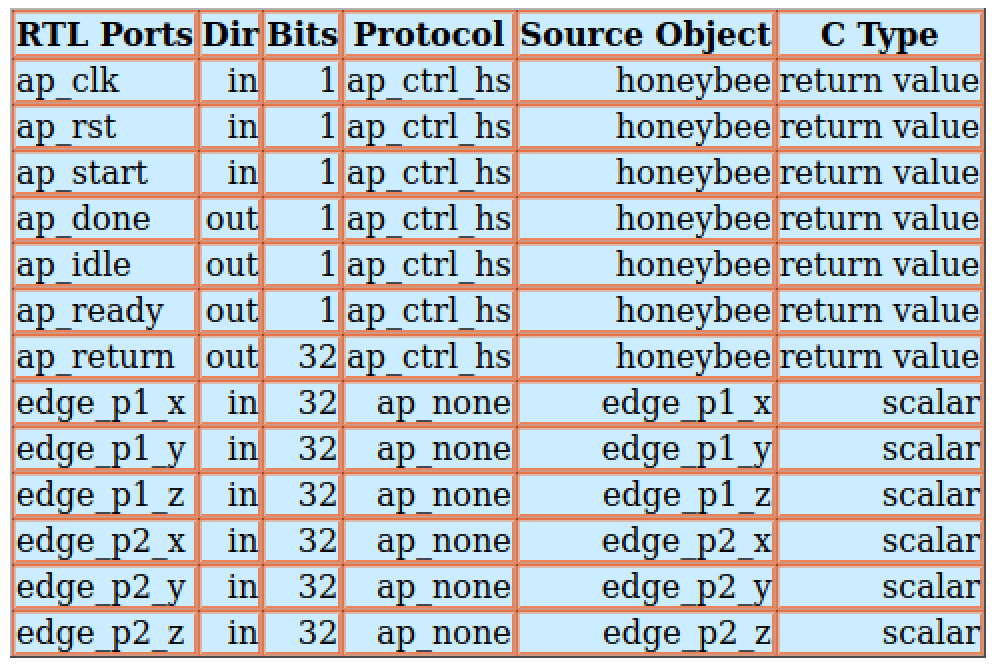
\includegraphics[width=0.9\linewidth]{chapters/chapter3/img/HB-A-synthesis.png}
    \caption{Interface Summary of HoneyBee-A Synthesis in Vivado HLS}
    \label{fig:HB-A-synthesis}
\end{center}
\end{figure}
\todo[inline]{Turn this into a table or get image from vivado}
    
    \subsection{Measurement and Analysis}
        \subsubsection*{HoneyBee-A}
            The synthesis results of HoneyBee-A are shown in Table \ref{table:HBA}. It compares the execution time in microseconds for one edge to undergo collision detection if software and then in different synthesis ``solutions''. MacOS and Ubuntu executing the function defined in honeybee.c have fairly similar results. Solution 1, which is the synthesized version of honeybee.c without any pipelining, was significantly slower. This is to be expected, as both MacOS and Ubuntu, operating on intel processors, would likely have some degree of pipelining and optimization of executing the compiled C code. However, significant improvements are observed once pipelining is implemented. Solutions 2-4 are increasing amounts of pipelining. Across the board, solutions 3 and 4 are roughly equal, but significantly faster that both solution 1 and the MacOS/Ubuntu execution times. Solution 4 shows a speedup of over 10x MacOS and Ubuntu.
            \begin{table}[H]
\begin{center}
\begin{tabular}{|m{0.13\linewidth}|m{0.11\linewidth}|m{0.11\linewidth}|m{0.1\linewidth}|m{0.1\linewidth}|m{0.1\linewidth}|m{0.1\linewidth}|}
\hline
Dimensions   & Mac OS & Ubuntu & 1 & 2 & 3 & 4 \\
\hline
4x4x4       & 2 & 2 & 21.6 & 1.5 & 0.44 & 0.47 \\
8x8x8       & 23 & 19 & 151 & 5.53 & 2.2 & 1.79 \\
16x16x16    & 166 & 180 & 1133 & 41.37 & 13.08 & 12.11 \\
32x32x32    & 1317 & 1424 & 8783 & 328 & 103 & 104 \\
\hline
\end{tabular}
\caption{Simulated performance of HB-A in microseconds}
\label{tables:HBA}
\end{center}
\end{table}

            When HoneyBee-A is simulated in full \gls{RRT} execution, we see similarly promising results. Table \ref{table:rrt-with-hba} shows the results of simulated RRT execution with HoneyBee-A. This is also shown in Figure \ref{fig:rrt-with-hba}.
            % @Author: AnthonyKenny98
% @Date:   2020-02-29 22:26:11
% @Last Modified by:   AnthonyKenny98
% @Last Modified time: 2020-02-29 22:26:11

            % @Author: AnthonyKenny98
% @Date:   2020-02-29 22:26:11
% @Last Modified by:   AnthonyKenny98
% @Last Modified time: 2020-02-29 22:26:11


            \todo[inline]{Expand Discussion of HoneyBee-A Results}